\section{Results on Multiple Video Sequences}
\label{sec:results/section_a}

Running the experiment with all the possible combinations of QP and MSR as shown in Table \ref{tab:qp_msr_range}, we obtained the result from all 12 video sequences. For each pair of QP and MSR, we averaged each score across all 12 video sequences. As there are 20 metrics for evaluating object tracking performance, and MOTA is a good indicator of the overall tracking performance as explained in Chapter \ref{sec:background/section_d}, we focused our study on MOTA. In the following analysis, we visualized the data and conducted a regression analysis and t-test to quantify the results. Note that the methodologies of statistical analysis we employed are from the textbook \cite{kutner_applied_2005}.

% ----------------------------------------------------------
% Visualization
% ----------------------------------------------------------

\subsection{Visualization of All Video Sequences}
\label{subsec:/results/section_a/visualization}
We visualized MOTA score for "all" object classes across all video sequences at different QP and MSR as shown in Figure \ref{fig:averaged_result_all_qp}.
\begin{figure}[!htbp]
  \centering
  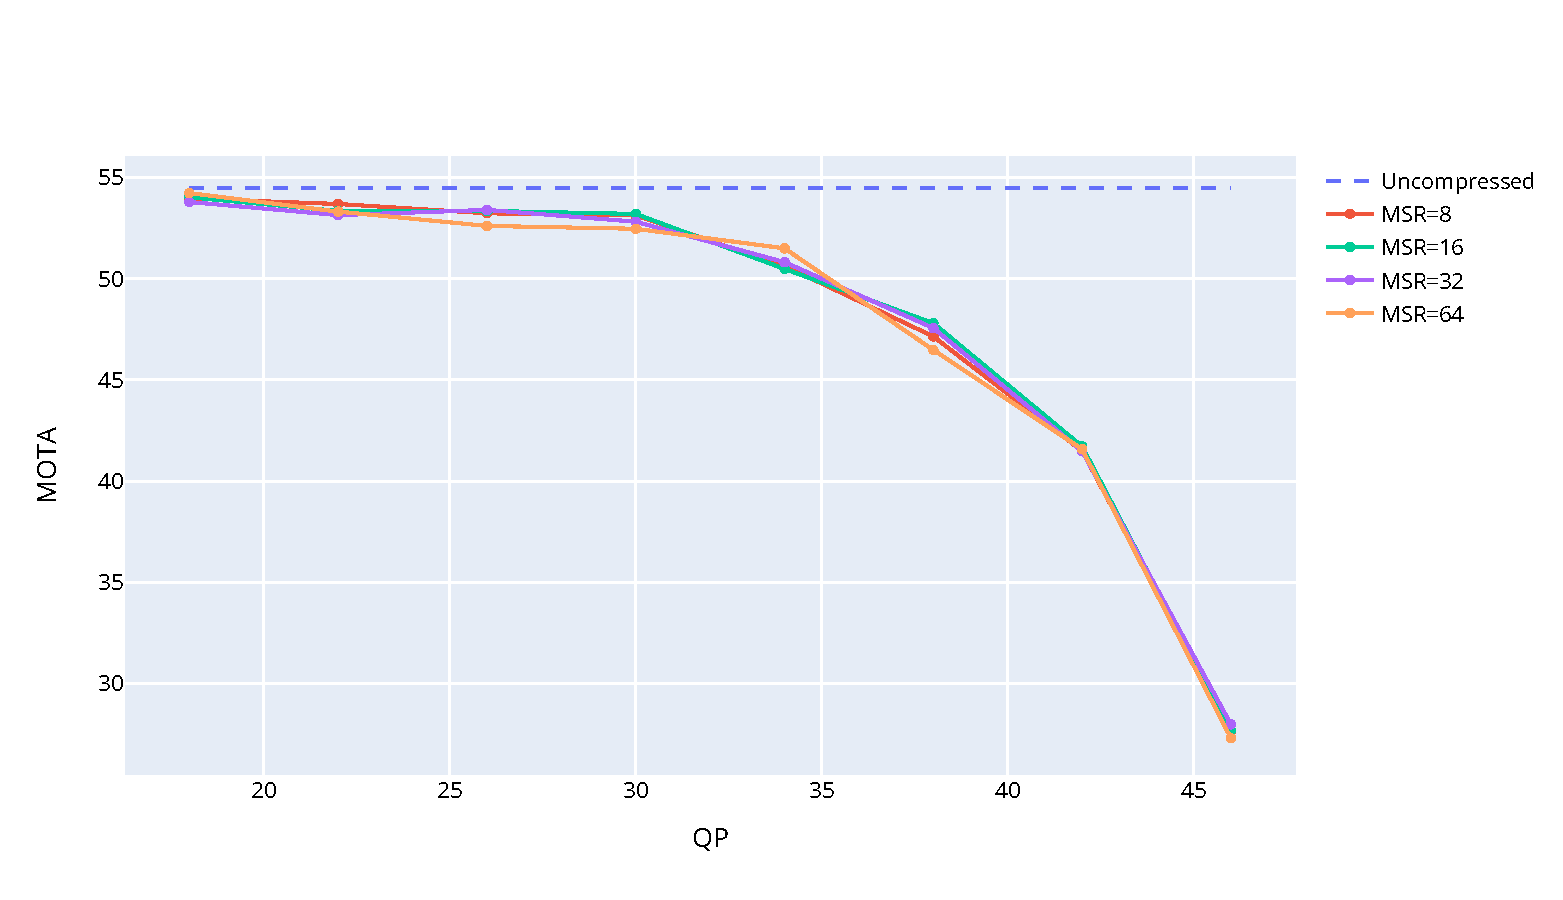
\includegraphics[width=1.0\linewidth]{img/averaged_result_all_qp.pdf}
  \caption[Averaged Result of All Video Samples with All Object Classes]{
    
  }
  \label{fig:averaged_result_all_qp}
\end{figure}
As can be seen from the plot, the uncompressed video sequences achieved the highest MOTA score. For the compressed sequences, the MOTA score is lower than the uncompressed result, and the higher the QP, the lower the MOTA score. Although the scores at different MSR are shown, we do not see any significant differences between MOTA scores at different MSR values from this plot. Not only MOTA, we observed that the performance scores of most of the other metrics decrease as QP increases.

Figure \ref{fig:averaged_result_all_multiplots_qp} shows the visualization of all the metrics over different QP and MSR, and Table \ref{tab:averaged_result_all} tabulates their values. Note that the metric GT is omitted from the visualization since it is a constant value, and the value can be confirmed from the table. 
\begin{figure}[!htbp]
  \centering
  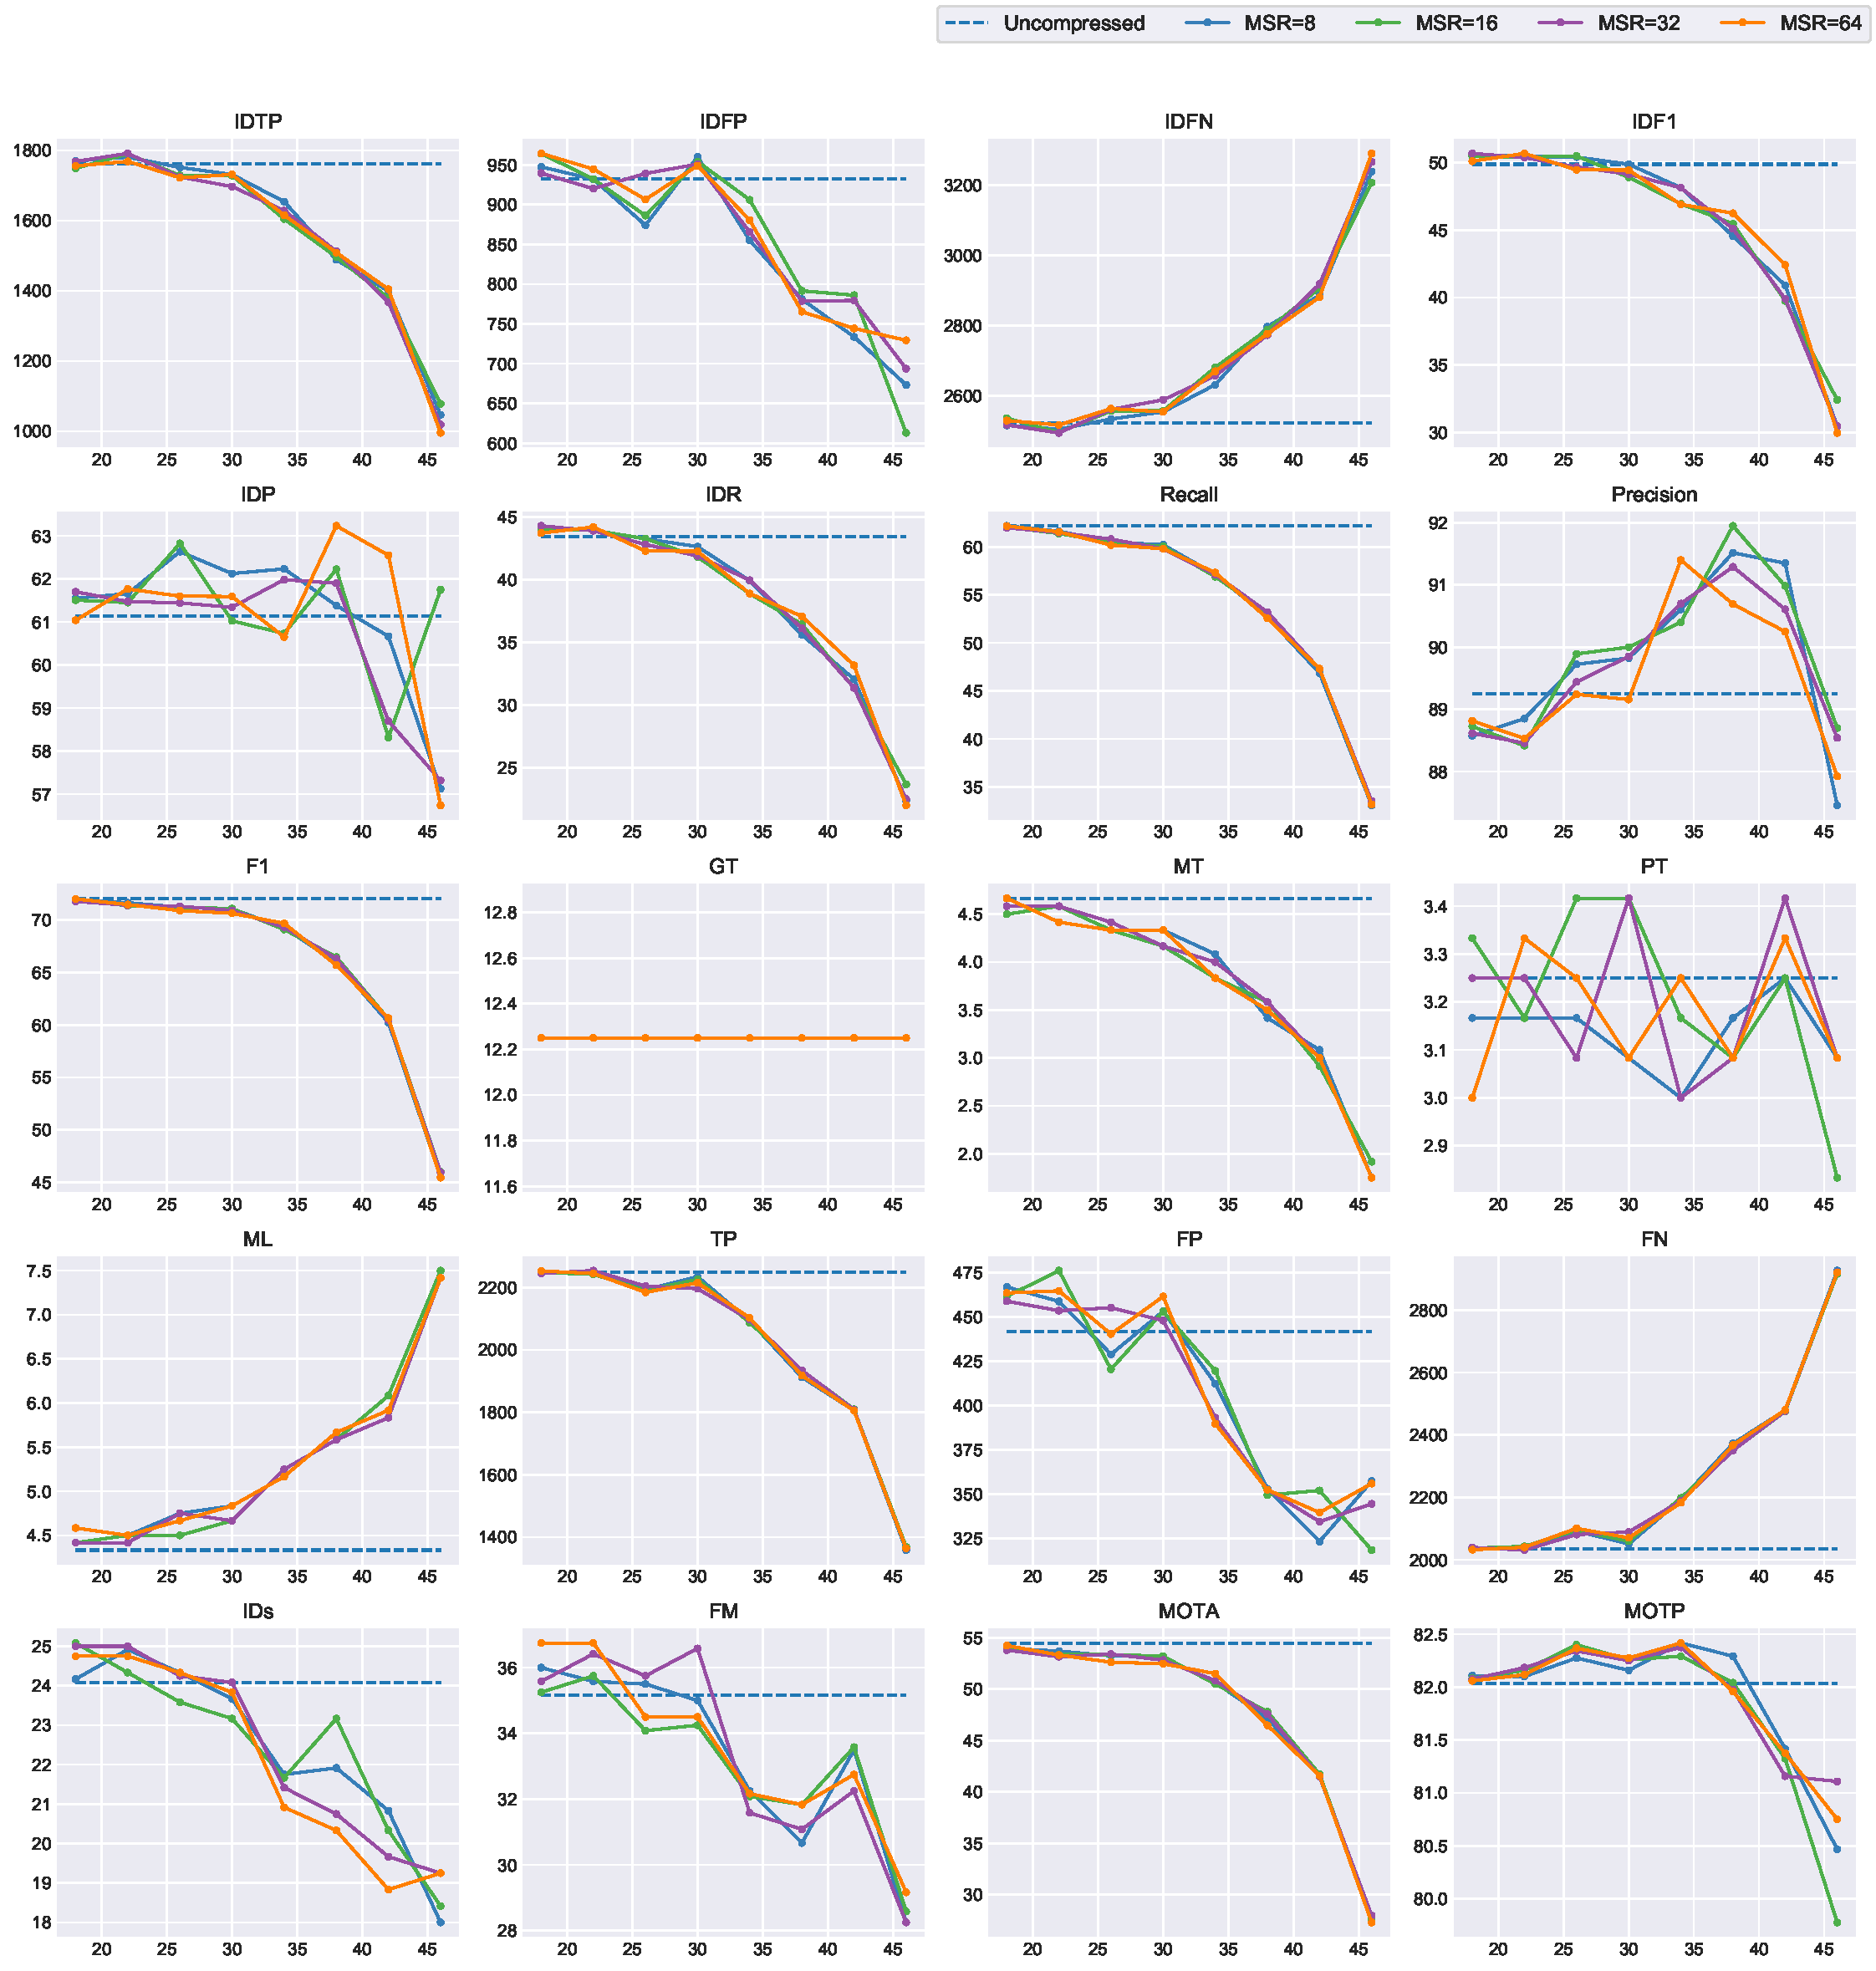
\includegraphics[width=1.0\linewidth]{img/averaged_all_multiplots_qp.pdf}
  \caption[Averaged Result of All Video Samples with All Object Classes]{
    
  }
  \label{fig:averaged_result_all_multiplots_qp}
\end{figure}
\begin{table}[!htbp]
  \centering
  \caption[Averaged performance results of all video samples]
  {Averaged performance results of all video samples.}

  % table for uncompressed
  \begin{subtable}[t]{\linewidth}
    \centering
    \vspace{0pt}
    \resizebox{1.0\linewidth}{!}{
    \begin{tabular}{llrrrrrrrrrrrrrrrrrrrr}
    \toprule
              QP &          MSR &    IDTP &   IDFP &    IDFN &  IDF1 &   IDP &   IDR &  Recall &  Precision &    F1 &    GT &   MT &   PT &   ML &      TP &     FP &      FN &   IDs &    FM &  MOTA &  MOTP \\
    \midrule
    Uncompressed & Uncompressed & 1762.58 & 932.83 & 2522.67 & 49.88 & 61.13 & 43.48 &   62.17 &      89.25 & 72.08 & 12.25 & 4.67 & 3.25 & 4.33 & 2249.75 & 441.67 & 2035.50 & 24.08 & 35.17 & 54.49 & 82.03 \\
    \bottomrule
    \end{tabular}}
    \caption{Mean values for the uncompressed sequence}
  \end{subtable}
 
 
 
  
  % table for msr=8
  \begin{subtable}[t]{\linewidth}
    \centering
    \resizebox{1.0\linewidth}{!}{
    \begin{tabular}{rrrrrrrrrrrrrrrrrrrrrr}
    \toprule
     QP &  MSR &    IDTP &   IDFP &    IDFN &  IDF1 &   IDP &   IDR &  Recall &  Precision &    F1 &    GT &   MT &   PT &   ML &      TP &     FP &      FN &   IDs &    FM &  MOTA &  MOTP \\
    \midrule
     18 &    8 & 1770.08 & 947.50 & 2515.17 & 50.60 & 61.55 & 44.26 &   62.18 &      88.58 & 71.92 & 12.25 & 4.50 & 3.17 & 4.58 & 2246.75 & 466.83 & 2038.50 & 24.17 & 36.00 & 53.97 & 82.11 \\
     22 &    8 & 1780.83 & 931.92 & 2504.42 & 50.46 & 61.66 & 43.96 &   61.62 &      88.85 & 71.65 & 12.25 & 4.58 & 3.17 & 4.50 & 2250.00 & 458.75 & 2035.25 & 24.92 & 35.58 & 53.70 & 82.10 \\
     26 &    8 & 1751.67 & 874.17 & 2533.58 & 50.41 & 62.63 & 43.28 &   60.49 &      89.73 & 71.22 & 12.25 & 4.33 & 3.17 & 4.75 & 2192.92 & 428.92 & 2092.33 & 24.33 & 35.50 & 53.24 & 82.28 \\
     30 &    8 & 1731.50 & 960.08 & 2553.75 & 49.88 & 62.12 & 42.65 &   60.21 &      89.83 & 71.07 & 12.25 & 4.33 & 3.08 & 4.83 & 2234.42 & 453.17 & 2050.83 & 23.67 & 35.00 & 53.13 & 82.16 \\
     34 &    8 & 1653.92 & 855.08 & 2631.33 & 48.14 & 62.23 & 39.93 &   57.12 &      90.61 & 69.26 & 12.25 & 4.08 & 3.00 & 5.17 & 2092.58 & 412.42 & 2192.67 & 21.75 & 32.25 & 50.64 & 82.42 \\
     38 &    8 & 1488.50 & 781.08 & 2796.75 & 44.56 & 61.38 & 35.62 &   52.70 &      91.52 & 65.97 & 12.25 & 3.42 & 3.17 & 5.67 & 1912.42 & 353.17 & 2372.83 & 21.92 & 30.67 & 47.15 & 82.29 \\
     42 &    8 & 1399.25 & 733.83 & 2886.00 & 40.92 & 60.67 & 32.08 &   46.86 &      91.35 & 60.24 & 12.25 & 3.08 & 3.25 & 5.92 & 1805.67 & 323.42 & 2479.58 & 20.83 & 33.50 & 41.48 & 81.42 \\
     46 &    8 & 1046.50 & 673.33 & 3238.75 & 30.48 & 57.12 & 22.40 &   33.09 &      87.46 & 45.48 & 12.25 & 1.75 & 3.08 & 7.42 & 1358.33 & 357.50 & 2926.92 & 18.00 & 28.25 & 27.64 & 80.47 \\
    \bottomrule
    \end{tabular}}
    \caption{Mean values for MSR = 8}
  \end{subtable}
 
 
  
  % table for msr=16
  \begin{subtable}[t]{\linewidth}
    \centering
    \resizebox{1.0\linewidth}{!}{
    \begin{tabular}{rrrrrrrrrrrrrrrrrrrrrr}
    \toprule
     QP &  MSR &    IDTP &   IDFP &    IDFN &  IDF1 &   IDP &   IDR &  Recall &  Precision &    F1 &    GT &   MT &   PT &   ML &      TP &     FP &      FN &   IDs &    FM &  MOTA &  MOTP \\
    \midrule
     18 &   16 & 1749.25 & 964.25 & 2536.00 & 50.48 & 61.51 & 44.07 &   62.04 &      88.73 & 71.88 & 12.25 & 4.50 & 3.33 & 4.42 & 2248.00 & 461.50 & 2037.25 & 25.08 & 35.25 & 54.03 & 82.08 \\
     22 &   16 & 1790.08 & 932.17 & 2495.17 & 50.40 & 61.45 & 43.96 &   61.39 &      88.42 & 71.38 & 12.25 & 4.58 & 3.17 & 4.50 & 2242.17 & 476.08 & 2043.08 & 24.33 & 35.75 & 53.36 & 82.16 \\
     26 &   16 & 1728.75 & 886.25 & 2556.50 & 50.48 & 62.82 & 43.28 &   60.43 &      89.89 & 71.21 & 12.25 & 4.33 & 3.42 & 4.50 & 2190.50 & 420.50 & 2094.75 & 23.58 & 34.08 & 53.36 & 82.40 \\
     30 &   16 & 1728.33 & 954.08 & 2556.92 & 48.91 & 61.02 & 41.83 &   60.04 &      90.00 & 71.10 & 12.25 & 4.17 & 3.42 & 4.67 & 2225.42 & 453.00 & 2059.83 & 23.17 & 34.25 & 53.21 & 82.26 \\
     34 &   16 & 1604.67 & 906.00 & 2680.58 & 46.94 & 60.73 & 38.90 &   56.89 &      90.40 & 69.10 & 12.25 & 3.83 & 3.17 & 5.25 & 2087.08 & 419.58 & 2198.17 & 21.67 & 32.08 & 50.49 & 82.29 \\
     38 &   16 & 1496.58 & 791.58 & 2788.67 & 45.47 & 62.23 & 36.46 &   53.13 &      91.95 & 66.47 & 12.25 & 3.58 & 3.08 & 5.58 & 1934.58 & 349.58 & 2350.67 & 23.17 & 31.83 & 47.81 & 82.04 \\
     42 &   16 & 1379.33 & 786.17 & 2905.92 & 39.76 & 58.32 & 31.38 &   47.28 &      90.98 & 60.56 & 12.25 & 2.92 & 3.25 & 6.08 & 1809.33 & 352.17 & 2475.92 & 20.33 & 33.58 & 41.72 & 81.33 \\
     46 &   16 & 1078.17 & 613.00 & 3207.08 & 32.42 & 61.75 & 23.68 &   33.48 &      88.70 & 45.99 & 12.25 & 1.92 & 2.83 & 7.50 & 1368.58 & 318.58 & 2916.67 & 18.42 & 28.58 & 27.67 & 79.77 \\
    \bottomrule
    \end{tabular}}
    \caption{Mean values for MSR = 16}
  \end{subtable}
 
 
 
  % table for msr=32
  \begin{subtable}[t]{\linewidth}
    \centering
    \resizebox{1.0\linewidth}{!}{
    \begin{tabular}{rrrrrrrrrrrrrrrrrrrrrr}
    \toprule
     QP &  MSR &    IDTP &   IDFP &    IDFN &  IDF1 &   IDP &   IDR &  Recall &  Precision &    F1 &    GT &   MT &   PT &   ML &      TP &     FP &      FN &   IDs &    FM &  MOTA &  MOTP \\
    \midrule
     18 &   32 & 1768.58 & 939.58 & 2516.67 & 50.67 & 61.70 & 44.31 &   61.98 &      88.62 & 71.78 & 12.25 & 4.58 & 3.25 & 4.42 & 2245.33 & 458.83 & 2039.92 & 25.00 & 35.58 & 53.80 & 82.08 \\
     22 &   32 & 1791.42 & 920.08 & 2493.83 & 50.38 & 61.48 & 43.92 &   61.49 &      88.46 & 71.42 & 12.25 & 4.58 & 3.25 & 4.42 & 2254.00 & 453.50 & 2031.25 & 25.00 & 36.42 & 53.15 & 82.18 \\
     26 &   32 & 1724.42 & 939.08 & 2560.83 & 49.68 & 61.44 & 42.82 &   60.80 &      89.44 & 71.32 & 12.25 & 4.42 & 3.08 & 4.75 & 2204.33 & 455.17 & 2080.92 & 24.25 & 35.75 & 53.41 & 82.34 \\
     30 &   32 & 1697.08 & 950.92 & 2588.17 & 49.14 & 61.34 & 41.91 &   59.79 &      89.85 & 70.91 & 12.25 & 4.17 & 3.42 & 4.67 & 2196.08 & 447.92 & 2089.17 & 24.08 & 36.58 & 52.83 & 82.25 \\
     34 &   32 & 1628.42 & 865.50 & 2656.83 & 48.13 & 61.98 & 39.98 &   57.10 &      90.70 & 69.32 & 12.25 & 4.00 & 3.00 & 5.25 & 2096.75 & 393.17 & 2188.50 & 21.42 & 31.58 & 50.83 & 82.38 \\
     38 &   32 & 1512.50 & 778.75 & 2772.75 & 45.10 & 61.90 & 36.13 &   53.20 &      91.29 & 66.31 & 12.25 & 3.58 & 3.08 & 5.58 & 1934.67 & 352.58 & 2350.58 & 20.75 & 31.08 & 47.57 & 81.98 \\
     42 &   32 & 1367.25 & 779.58 & 2918.00 & 39.92 & 58.70 & 31.38 &   47.28 &      90.61 & 60.48 & 12.25 & 3.00 & 3.42 & 5.83 & 1808.25 & 334.58 & 2477.00 & 19.67 & 32.25 & 41.48 & 81.16 \\
     46 &   32 & 1018.67 & 693.75 & 3266.58 & 30.47 & 57.32 & 22.52 &   33.53 &      88.54 & 45.93 & 12.25 & 1.75 & 3.08 & 7.42 & 1363.75 & 344.67 & 2921.50 & 19.25 & 28.25 & 27.97 & 81.11 \\
    \bottomrule
    \end{tabular}}
    \caption{Mean values for MSR = 32}
  \end{subtable}
  
  
  % table for msr=64
  \begin{subtable}[t]{\linewidth}
    \centering
    \resizebox{1.0\linewidth}{!}{
    \begin{tabular}{rrrrrrrrrrrrrrrrrrrrrr}
    \toprule
     QP &  MSR &    IDTP &   IDFP &    IDFN &  IDF1 &   IDP &   IDR &  Recall &  Precision &    F1 &    GT &   MT &   PT &   ML &      TP &     FP &      FN &   IDs &    FM &  MOTA &  MOTP \\
    \midrule
     18 &   64 & 1756.00 & 964.33 & 2529.25 & 50.10 & 61.04 & 43.73 &   62.17 &      88.82 & 72.02 & 12.25 & 4.67 & 3.00 & 4.58 & 2252.83 & 463.50 & 2032.42 & 24.75 & 36.75 & 54.24 & 82.06 \\
     22 &   64 & 1768.75 & 944.75 & 2516.50 & 50.68 & 61.77 & 44.22 &   61.56 &      88.53 & 71.48 & 12.25 & 4.42 & 3.33 & 4.50 & 2244.83 & 464.67 & 2040.42 & 24.75 & 36.75 & 53.33 & 82.12 \\
     26 &   64 & 1722.25 & 906.50 & 2563.00 & 49.46 & 61.60 & 42.30 &   60.18 &      89.24 & 70.90 & 12.25 & 4.33 & 3.25 & 4.67 & 2184.42 & 440.33 & 2100.83 & 24.33 & 34.50 & 52.62 & 82.37 \\
     30 &   64 & 1731.25 & 949.00 & 2554.00 & 49.44 & 61.59 & 42.27 &   59.80 &      89.16 & 70.64 & 12.25 & 4.33 & 3.08 & 4.83 & 2214.75 & 461.50 & 2070.50 & 23.83 & 34.50 & 52.47 & 82.28 \\
     34 &   64 & 1615.58 & 880.42 & 2669.67 & 46.90 & 60.65 & 38.91 &   57.32 &      91.40 & 69.69 & 12.25 & 3.83 & 3.25 & 5.17 & 2102.25 & 389.75 & 2183.00 & 20.92 & 32.17 & 51.51 & 82.42 \\
     38 &   64 & 1508.92 & 765.42 & 2776.33 & 46.25 & 63.23 & 37.09 &   52.56 &      90.69 & 65.69 & 12.25 & 3.50 & 3.08 & 5.67 & 1917.75 & 352.58 & 2367.50 & 20.33 & 31.83 & 46.48 & 81.96 \\
     42 &   64 & 1404.50 & 744.42 & 2880.75 & 42.43 & 62.55 & 33.18 &   47.31 &      90.25 & 60.65 & 12.25 & 3.00 & 3.33 & 5.92 & 1805.17 & 339.75 & 2480.08 & 18.83 & 32.75 & 41.57 & 81.38 \\
     46 &   64 &  995.00 & 729.42 & 3290.25 & 29.98 & 56.74 & 22.02 &   33.18 &      87.92 & 45.43 & 12.25 & 1.75 & 3.08 & 7.42 & 1364.33 & 356.08 & 2920.92 & 19.25 & 29.17 & 27.29 & 80.75 \\
    \bottomrule
    \end{tabular}}
    \caption{Mean values for MSR = 64}
  \end{subtable}

  
\label{tab:averaged_result_all}  
\end{table}
As discussed in Chapter \ref{sec:background/section_e}, the higher the QP, the lower the bitrate, so we expected the tracking performance to be lower. Our performance results from most metrics are consistent with this expectation. To explain the decrease of MOTA defined in terms of FP, FN, and IDs based on Equation \eqref{eqn:MOTA}, we can see that as QP increases, FP and IDs decreases but FN increases, which is consistent with our expectation. Although the decrease of FP and IDs contribute to the increase of MOTA, the increase of FN is significantly larger than FP and IDs; thus, MOTA decreases. However, we observed that Precision and MOTP are not entirely consistent with our expectation and that the performance first increases and then decreases as QP is increased. Since video samples differ in resolution, frame rate, number of objects, and object classes, tracking performance is different. Due to the relatively small number of video samples, the standard deviation is relatively high around the average performance. we show standard deviations in Appendix \ref{sec:appendix/section_std_dev}. As another visual representation to see if MSR impacts the performance scores, we visualized each performance score on a different MSR as a horizontal axis, and we observed no significant dependence on MSR as shown in Figure \ref{fig:averaged_result_all_multiplots_msr}.
\begin{figure}[!htbp]
  \centering
  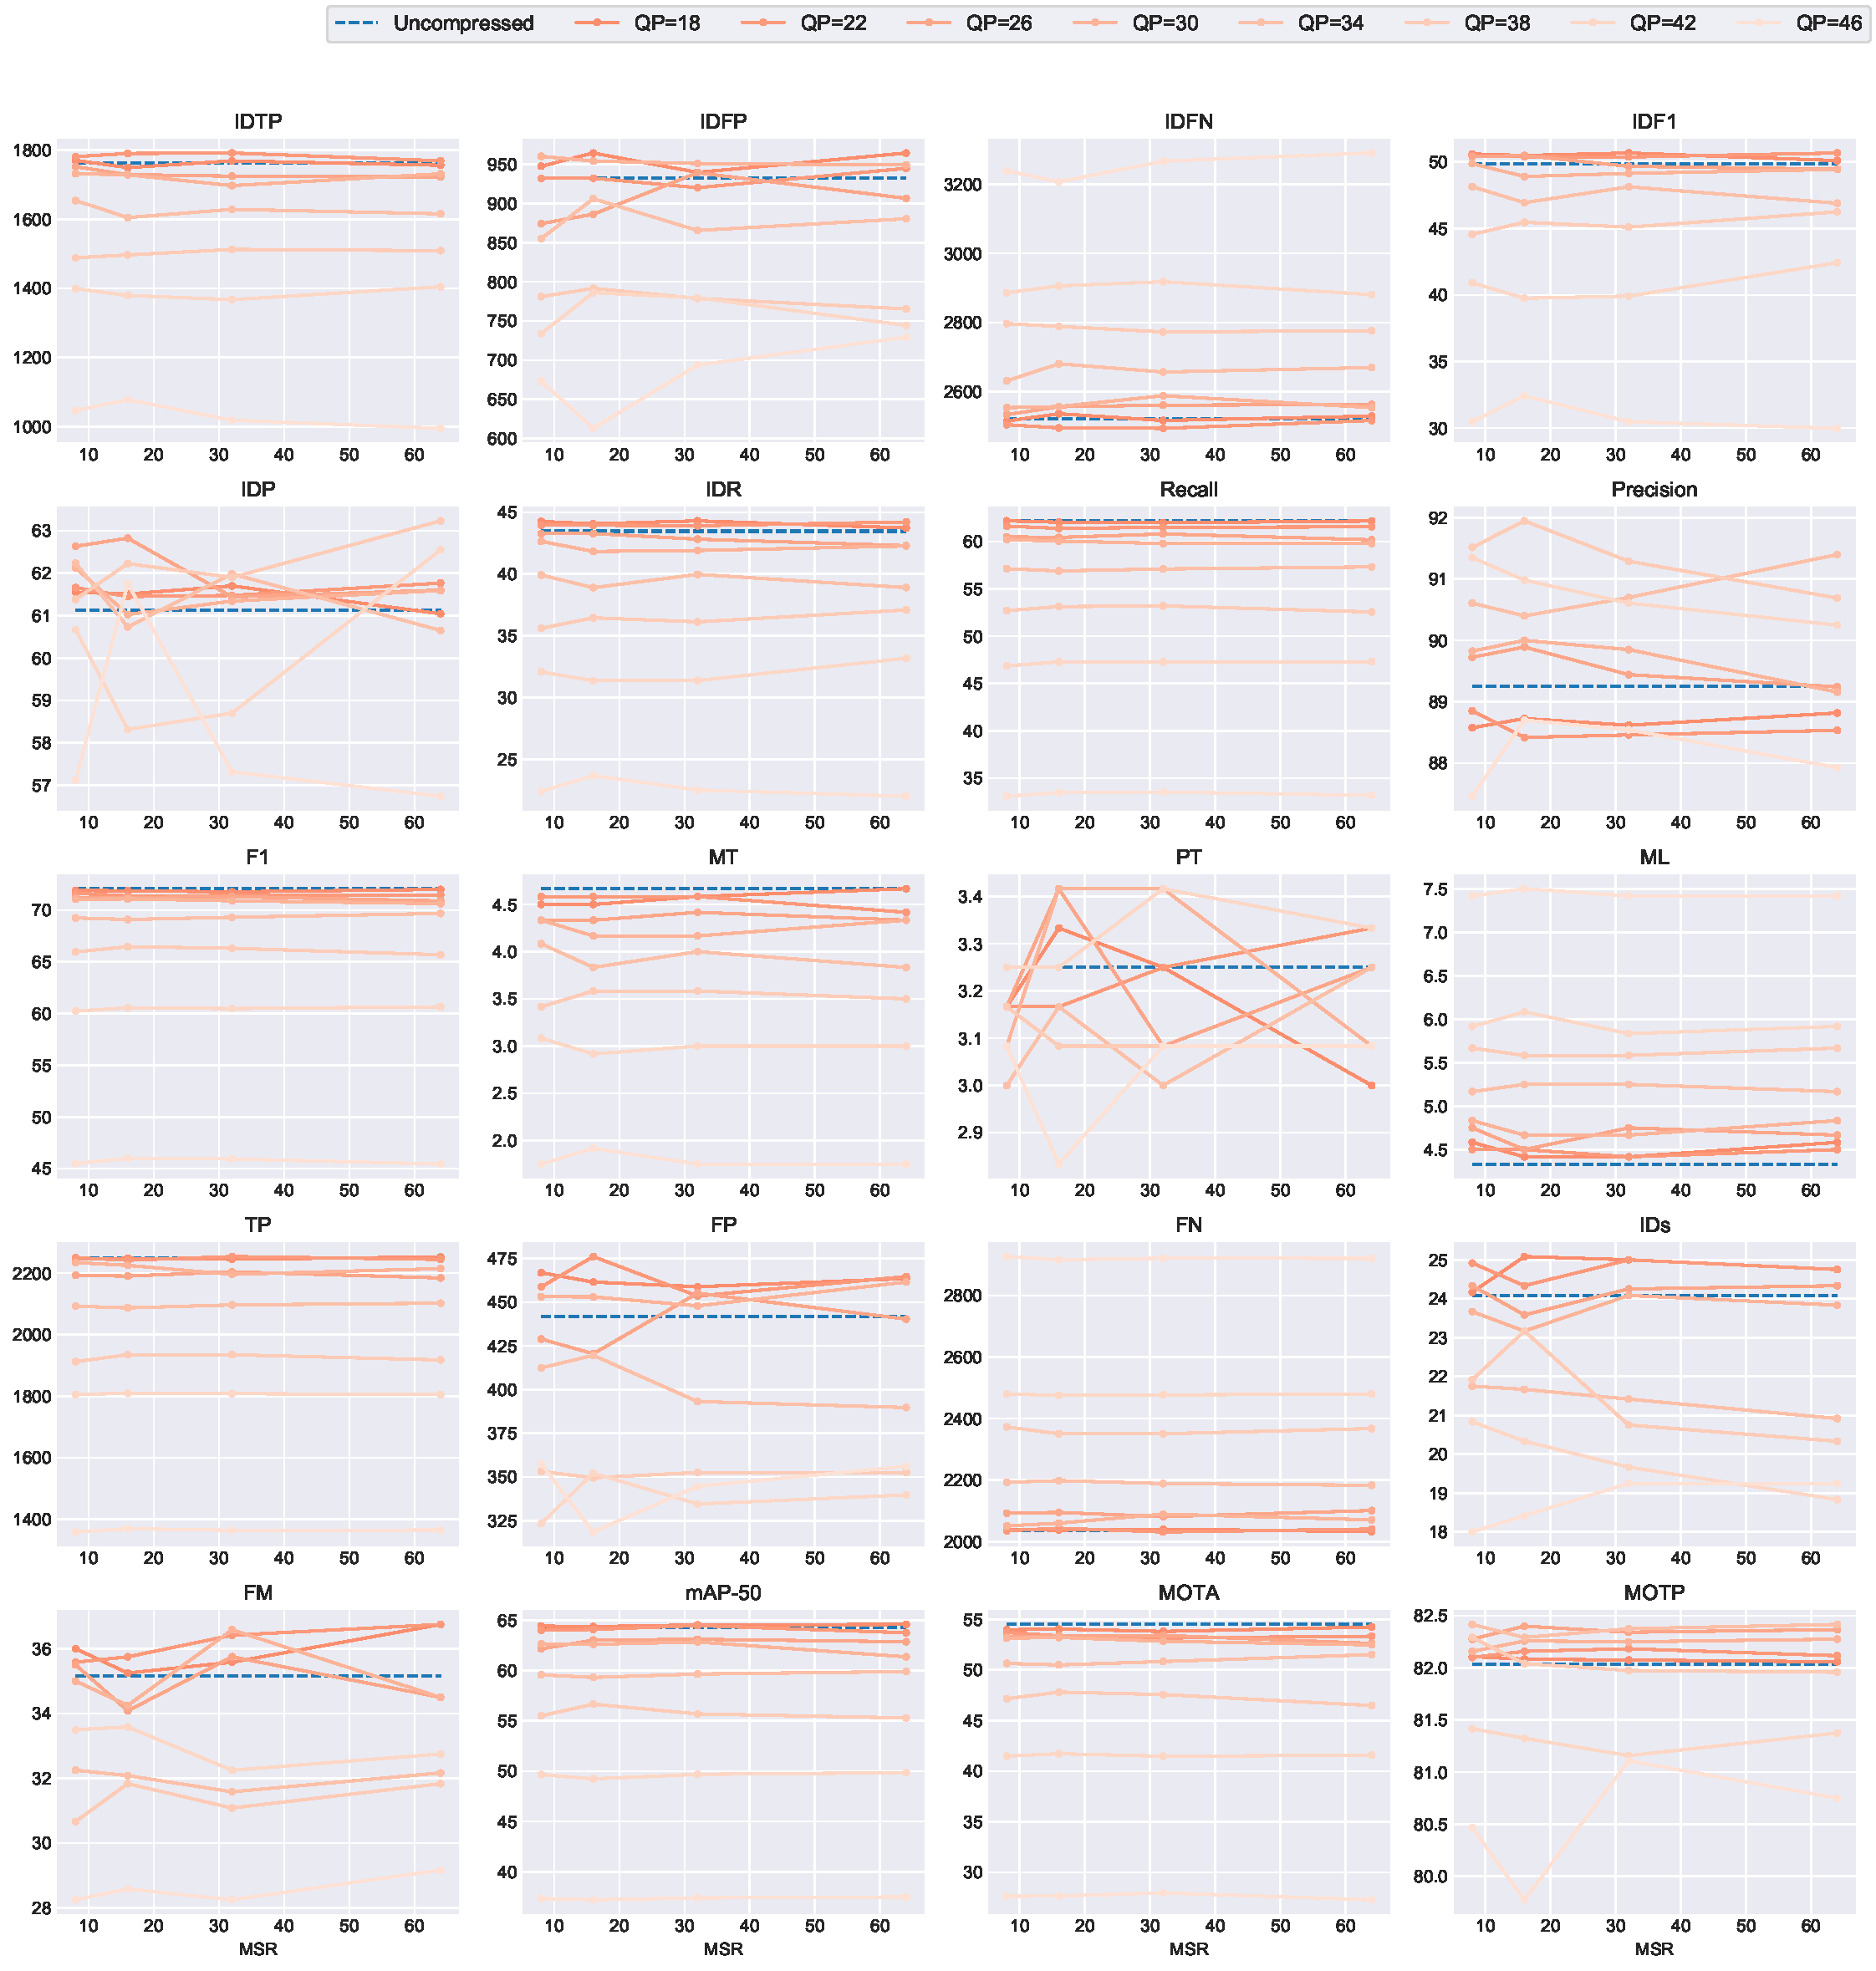
\includegraphics[width=1.0\linewidth]{img/averaged_all_multiplots_msr.pdf}
  \caption[Visualization of the averaged performance results at different MSR of all video samples]
  {Visualization of the average performance results at different MSR across all video samples.}
  \label{fig:averaged_result_all_multiplots_msr}
\end{figure}

% ----------------------------------------------------------
% Regression Analysis
% ----------------------------------------------------------

\subsection{Regression Analysis}
\label{subsec:/results/section_a/regression_analysis}
To examine the impact of QP and MSR on each metric score quantitatively, we conducted a regression analysis on the entire data (all the video sequences). As we focused on the analysis on the MOTA score, we quantified the result on MOTA over QP and MSR values. As can be seen from the visualization, the relationship between MOTA and MSR features constant, but QP shows non-linear. In order to conduct a linear regression analysis, we transformed QP so that the relationship between MOTA and $\text{QP}'$ features linear (we call the transformed QP as $\text{QP}'$). The determination of the form of QP transformation was found by plotting various forms on the scatter plots on the individual video sequences by trial and error. Figure \ref{fig:QP_transformation} shows the scatter plots of MOTA before and after the QP transformation on the example sequence BasketballPass. Using the form of Equation \eqref{eqn:QP_transformation}, the scatter plot of MOTA at different $\text{QP}'$ shows a linear relationship as shown in Figure \ref{fig:QP_transformation_after}. The similar outcomes were observed in the other video sequences.
% \begin{figure}[!tb]
%   \centering
%   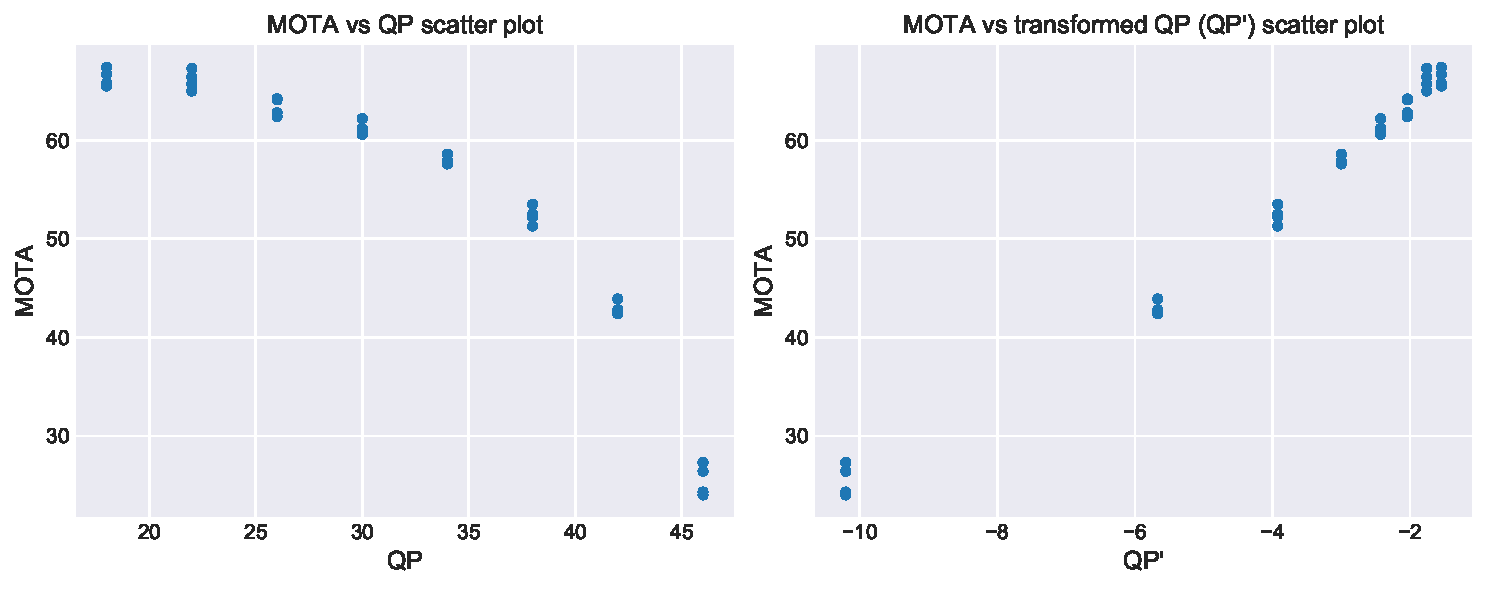
\includegraphics[width=1.0\linewidth]{img/QP_transformation.pdf}
%   \caption[Scatter plots before and after the QP transformation]
%   {Scatter plots before and after the QP transformation.}
%   \label{fig:QP_transformation}
% \end{figure}

\begin{figure}[!tb]
  \centering
  \begin{subfigure}[b]{.5\textwidth}
    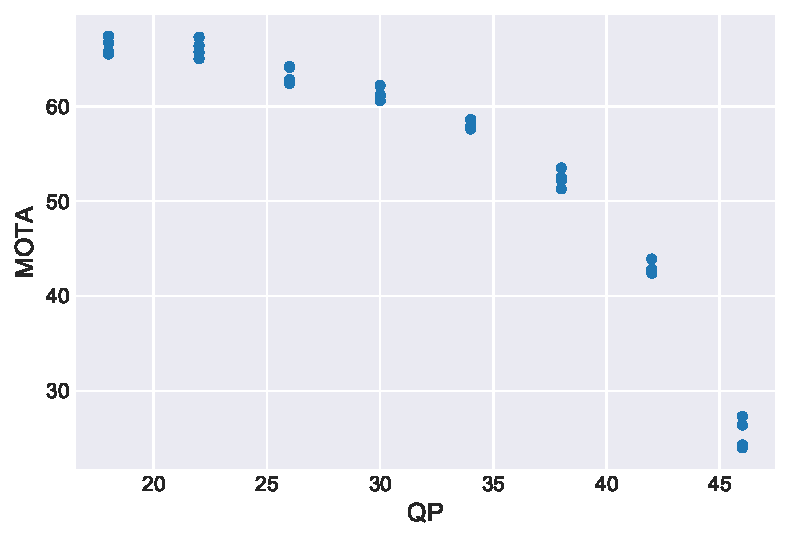
\includegraphics[width=\textwidth]{img/QP_transformation_before.pdf}
    \caption{MOTA vs QP scatter plot}
    \label{fig:QP_transformation_before}
  \end{subfigure}%
  \begin{subfigure}[b]{.5\textwidth}
    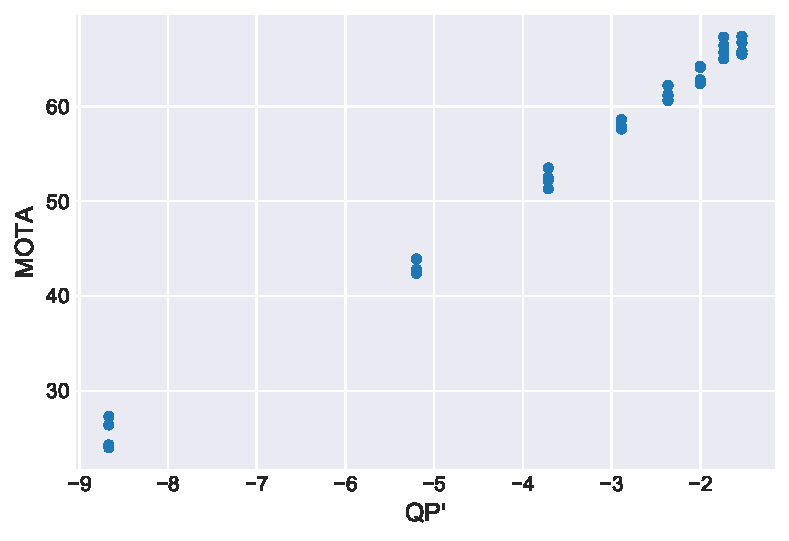
\includegraphics[width=\textwidth]{img/QP_transformation_after.pdf}
    \caption{MOTA vs $\text{QP}'$ scatter plot}
    \label{fig:QP_transformation_after}
  \end{subfigure}
  \caption[Scatter plots before and after the QP transformation on the BasketballPass sequence]{%
    Scatter plots before and after the QP transformation on the BasketballPass sequence.%
  }
  \label{fig:QP_transformation}
\end{figure}
\begin{equation}
\text{QP}' =  \frac{1}{\frac{\text{QP}}{51}-1}
\label{eqn:QP_transformation}
\end{equation}
However, using all the video sequences which have different level of the MOTA score, variance at each $\text{QP}'$ is high, and the little insight can be derived from the high variance of data as shown in Figure \ref{fig:MOTA_transformation_before}. Therefore, we transformed MOTA such that we subtract each MOTA score at different $\text{QP}'$ by the MOTA score at the uncompressed case, as represented below.
% \begin{figure}[!tb]
%   \centering
%   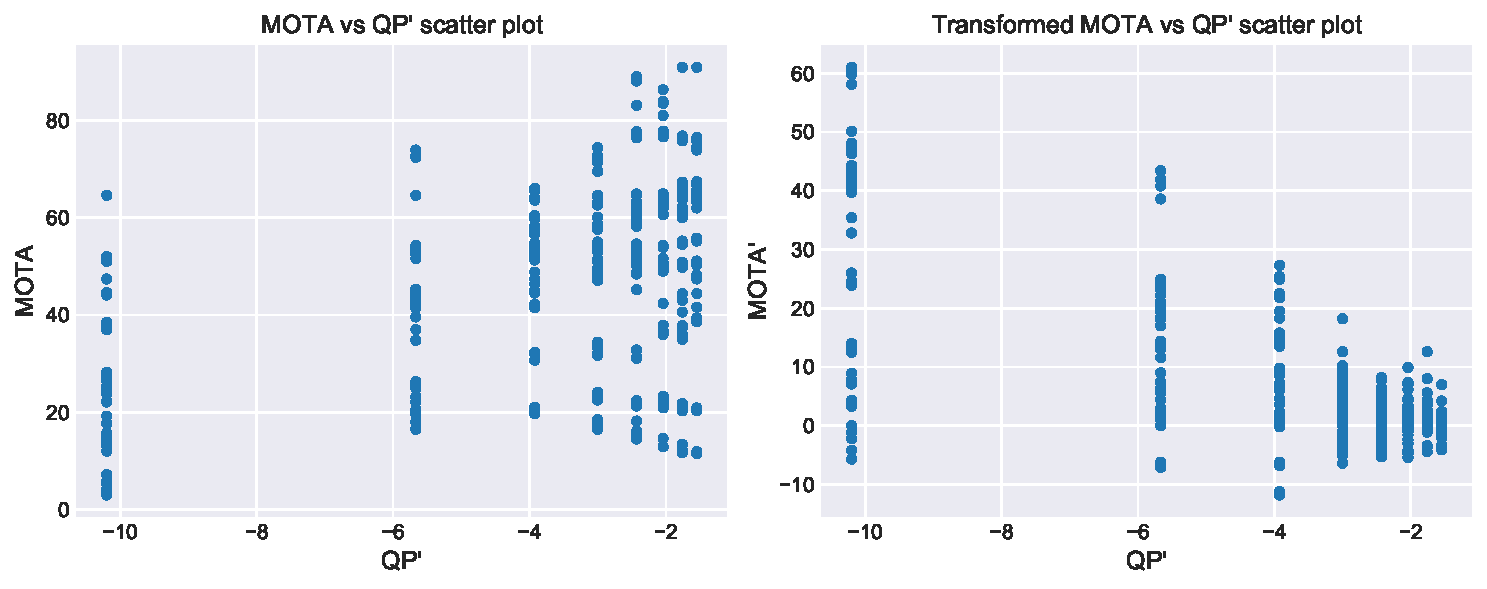
\includegraphics[width=1.0\linewidth]{img/MOTA_transformation.pdf}
%   \caption[Scatter plots before and after the MOTA transformation]
%   {Scatter plots before and after the MOTA transformation.}
%   \label{fig:MOTA_transformation}
% \end{figure}

% spacing between subfigures will not align the sub figures horizontanlly

\begin{figure}[!tb]
  \centering
  \begin{subfigure}{.5\linewidth}
    \centering
    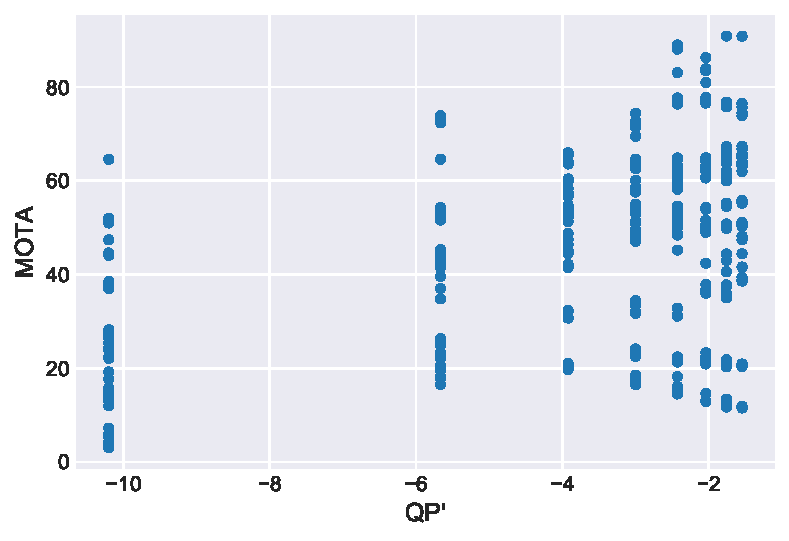
\includegraphics[width=\linewidth]{img/MOTA_transformation_before.pdf}
    \caption{MOTA vs $\text{QP}'$ scatter plot}
    \label{fig:MOTA_transformation_before}
  \end{subfigure}%
  \begin{subfigure}{.5\linewidth}
    \centering
    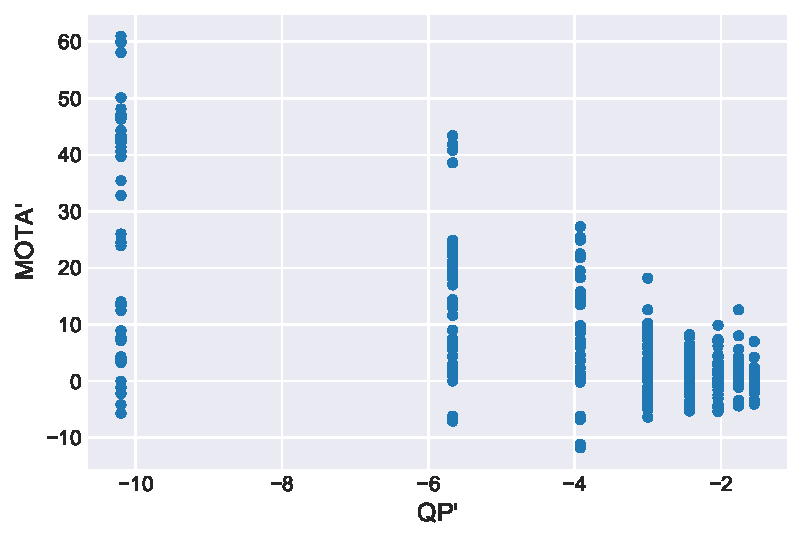
\includegraphics[width=\linewidth]{img/MOTA_transformation_after.pdf}
    \caption{$\text{MOTA}'$ vs $\text{QP}'$ scatter plot }
    \label{fig:MOTA_transformation_after}
  \end{subfigure}
  \caption[Scatter plots before and after the MOTA transformation on all the video sequences]{%
    Scatter plots before and after the MOTA transformation across all the video sequences.%
  }
  \label{fig:MOTA_transformation}
\end{figure}

\begin{equation}
\text{MOTA}' = \text{MOTA(Uncompressed)} -  \text{MOTA}(\text{QP}_i)
\label{eqn:MOTA_transformation}
\end{equation}
Doing this transformation, we can eliminate the bias from each video sequence but only consider the drop of the MOTA score from the uncompressed case. Figure \ref{fig:MOTA_transformation_after} shows the scatter plot of all the video sequences after the MOTA transformation. We can see from this figure that the relationship between $\text{MOTA}'$ and $\text{QP}'$ is still linear but error variance at each $\text{QP}'$ is not constant. Therefore, the weighted least squares method is appropriate in the regression model. Finally, since we have two continuous independent variables of $\text{QP}'$ and MSR and each may impact the continuous response variable of the $\text{MOTA}'$ score, we applied a multiple linear regression on all the video sequences. We represent the regression model as,
\begin{equation}
\text{MOTA}'_i = \beta_0 + \beta_1 \cdot \text{QP}'_i + \beta_2 \cdot \text{MSR}_i + \beta_3 \cdot \text{QP}'_i \cdot \text{MSR}_i + \epsilon_i~,
\label{eqn:regression_model}
\end{equation}
where $\beta_0$ is the intercept; $\beta_1$ and $\beta_2$ are the parameters of independent variables $\text{QP}'$ and MSR; $\beta_3$ is the parameter of the interaction term of $\text{QP}'$ and MSR. The interaction term is included to see if MSR and $\text{QP}'$ depend on each other. We assume that $\epsilon_i$ is the independent normally distributed error with mean 0 and variance $\sigma^2_i$. $i$ indicates the $i$-th trial from the independent variables. As we are applying the weighted least squares method, the weight at each $\text{QP}'$ can be calculated as
\begin{equation}
    w_i = \frac{1}{\sigma^2_i}
    \label{eqn:weight}
\end{equation}
Since $\sigma_i$ is the truth value of standard deviation at each $\text{QP}'$, we estimate $w_i$ using the sample standard deviation $s_i$ of data points at each $\text{QP}'$.

\setcounter{footnote}{1} % manully changing the footnote number. Referenced: https://tex.stackexchange.com/questions/359702/how-to-manually-reset-the-footnote-numbering-in-context
We utilized the Python package \cite{seabold_statsmodels_2010} for computation, and Table \ref{tab:regression} shows the results from the multiple linear regression analysis of the MOTA score\footnote{Each number only shows two decimal places, and -0.00 is not exactly zero but very small negative number. For 0.00, the value is very small positive number.}.
\begin{table}[!htbp]
    \centering
    \caption[Multiple linear regression analysis of averaged performance results]
    {Multiple linear regression analysis of averaged performance results.}
    \resizebox{1.0\linewidth}{!}{
\begin{tabular}{lrrrrrrrrrrrrrrrrrrr}
\toprule
{} &    IDTP &    IDFP &    IDFN &  IDF1 &   IDP &   IDR &  Recall &  Precision &    F1 &    MT &    PT &    ML &      TP &     FP &      FN &   IDs &    FM &  MOTA &  MOTP \\
\midrule
coefficient(Intercept) & 2312.69 & 1169.61 & 1972.56 & 65.29 & 64.37 & 60.56 &   82.86 &      88.28 & 90.22 &  6.55 &  3.41 &  2.30 & 2901.74 & 576.56 & 1383.51 & 29.18 & 40.46 & 72.71 & 83.54 \\
coefficient(QP)        &  -23.05 &  -10.07 &   23.05 & -0.62 & -0.10 & -0.71 &   -0.89 &       0.05 & -0.76 & -0.09 & -0.01 &  0.09 &  -27.78 &  -5.34 &   27.78 & -0.21 & -0.23 & -0.78 & -0.05 \\
coefficient(MSR)       &    0.10 &   -0.23 &   -0.10 & -0.02 & -0.01 & -0.02 &   -0.00 &       0.00 & -0.00 &  0.00 & -0.00 &  0.00 &   -0.06 &  -0.07 &    0.06 &  0.02 &  0.02 & -0.00 & -0.01 \\
coefficient(QP*MSR)    &   -0.01 &    0.01 &    0.01 &  0.00 &  0.00 &  0.00 &    0.00 &      -0.00 & -0.00 & -0.00 &  0.00 & -0.00 &    0.00 &   0.00 &   -0.00 & -0.00 & -0.00 & -0.00 &  0.00 \\
p-value(Intercept)     &    0.00 &    0.00 &    0.00 &  0.00 &  0.00 &  0.00 &    0.00 &       0.00 &  0.00 &  0.00 &  0.00 &  0.00 &    0.00 &   0.00 &    0.00 &  0.00 &  0.00 &  0.00 &  0.00 \\
p-value(QP)            &    0.00 &    0.00 &    0.00 &  0.00 &  0.05 &  0.00 &    0.00 &       0.21 &  0.00 &  0.00 &  0.13 &  0.00 &    0.00 &   0.00 &    0.00 &  0.00 &  0.00 &  0.00 &  0.00 \\
p-value(MSR)           &    0.98 &    0.87 &    0.98 &  0.88 &  0.74 &  0.88 &    0.98 &       0.93 &  0.99 &  0.89 &  0.42 &  0.89 &    0.99 &   0.91 &    0.99 &  0.54 &  0.62 &  1.00 &  0.73 \\
p-value(QP*MSR)        &    0.92 &    0.73 &    0.92 &  0.88 &  0.76 &  0.88 &    0.98 &       0.79 &  1.00 &  0.87 &  0.36 &  0.88 &    0.99 &   0.87 &    0.99 &  0.37 &  0.70 &  0.98 &  0.66 \\
\bottomrule
\end{tabular}
    }
    \label{tab:regression}
\end{table}
To see if the impact of the independent variable is statistically significant on the dependent variable, we conducted a hypothesis test at a significance level of 0.05. The null hypothesis is the case the parameter is 0 and the alternative hypothesis is the case the parameter is not zero.
\begin{equation}
    \begin{aligned}
        H_0: \beta_i = 0 \\
        H_1: \beta_i \neq 0 \\
    \end{aligned}
\end{equation}
From the table, the p-value for the test on QP is less than 0.05 while the p-values for the tests on MSR and the interaction term $\text{QP} \cdot \text{MSR}$ are greater than 0.05. This shows that we reject the null hypothesis of the test on QP, so QP significantly impacts MOTA at 95\% confidence. However, we fail to reject the null hypothesis for MSR and the interaction term of QP and MSR. Hence, the available data is insufficient to prove that MSR and the interaction term have statistically significant impact on the MOTA score. To justify these results, we tested the adequacy of our regression model with the normal probability plot of the residuals. To plot this, we would have to obtain the studentized residuals and the expected values of the studentized residuals under normality. The studentized residuals $e_i$ can be obtained as
\begin{equation}
    e_i = \frac{ \text{MOTA}'_{i,\text{measurement}} - \text{MOTA}'_{i,\text{predicted}} }{\sqrt{\text{MSE}_w}}
    \label{eqn:residuals}
\end{equation}
where $\text{MSE}_w$ is the weighted mean squared error.
\begin{equation}
    \text{MSE}_w = \frac{\sum w_i \cdot ( \text{MOTA}'_{i,\text{measurement}} - \text{MOTA}'_{i,\text{predicted}} )^2 }{n-4}
\end{equation}
$n$ is the number of measurements and we subtract by 4 since there are 4 parameters to estimate. The expected values of the studentized residuals under normality can be obtained from the following equation.
\begin{equation}
    \text{E}(e_i) = \sqrt{\text{MSE}_w} \cdot \text{ppf}( \frac{k - 0.375}{n + 0.25} )
\end{equation}
ppf is a percent point function (ppf) and $k$ is a rank of the residuals such that $k=1,2,3~..~n$. Figure \ref{fig:normal_probability_plot} shows the normal probability plot of studentized residuals and the expected values of the studentized residuals under normality.
\begin{figure}[!tb]
  \centering
  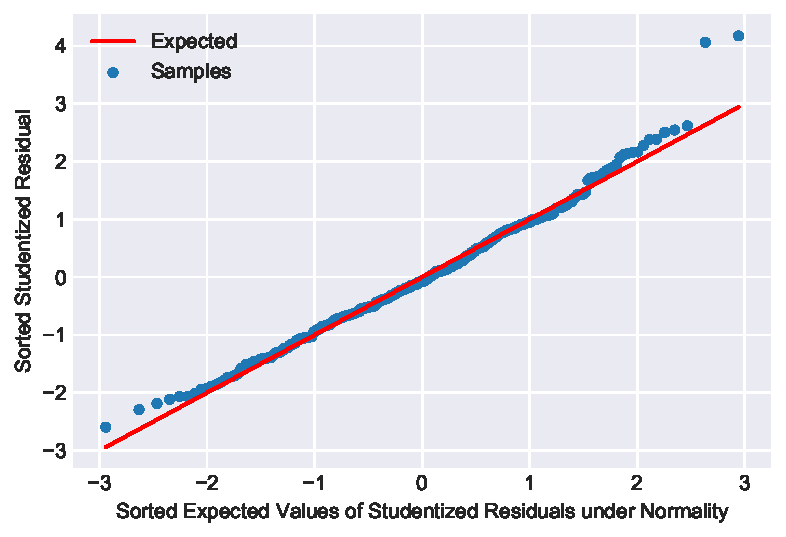
\includegraphics[width=0.8\linewidth]{img/normal_probability_plot.pdf}
  \caption[Normal probability plot to test the adequacy of the regression model]
  {Normal probability plot to test the adequacy of the regression model.}
  \label{fig:normal_probability_plot}
\end{figure}

Although we observe a slight departure from the normality which would be a straight line with a slope of 1.0, there is no major deviation from the straight line. Fitting this plot, we obtain a slope of 0.965 and the coefficient of determination $R^2$ of 0.922. The relatively high value of $R^2$ indicates that the error term $\epsilon_i$ is close to the normal distribution. Therefore, we conclude that our regression model \eqref{eqn:regression_model} is adequate. As we justified our regression model and from the hypothesis testing, We conclude that MSR does not impact the MOTA score, and QP and MSR do not depend on each other; therefore, our prediction for MSR, as explained in Chapter \ref{sec:background/section_e}, is inconsistent with our results. Thus, we will limit our further study to QP only.

% show the formulation
As we showed that our regression model \eqref{eqn:regression_model} is appropriate and therefore, we propose to formulate the relationship between MOTA and QP. From this regression, we have the following formulations.
\begin{equation}
    \text{MOTA}' = \beta_0 + \beta_1 \cdot \text{QP}'
\end{equation}
\begin{equation}
    \text{MOTA} = \text{MOTA(Uncompressed)} - \beta_0 - \beta_1 \cdot \frac{1}{ \frac{\text{QP}}{51} - 1 }
\label{eqn:MOTA_vs_QP_formula}
\end{equation}
Substituting the estimated values of parameters from Table \ref{tab:regression}, we have the following equation.
\begin{equation}
    \text{MOTA} = 58.32 + 2.64 \cdot \frac{1}{ \frac{\text{QP}}{51} - 1 }
\label{eqn:MOTA_vs_QP_formula_substituted}
\end{equation}
We plotted the average values of MOTA measurements at each QP and overlaid the fitted model \ref{eqn:MOTA_vs_QP_formula_substituted} on the scatter plot as shown in Figure \ref{fig:MOTA_vs_QP_formulation}.
\begin{figure}[!tb]
  \centering
  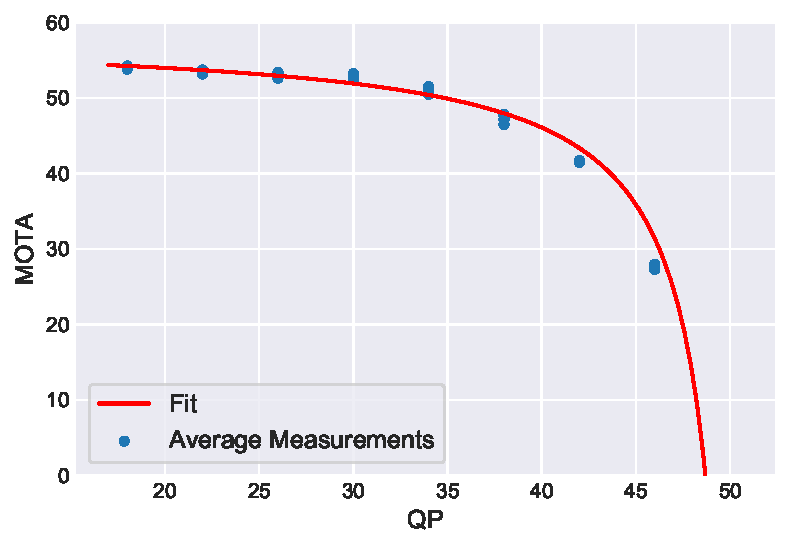
\includegraphics[width=0.8\linewidth]{img/MOTA_vs_QP_formulation.pdf}
  \caption[Scatter plot of average values of MOTA measurements and fitted model]
  {Scatter plot of average values of MOTA measurements and fitted model.}
  \label{fig:MOTA_vs_QP_formulation}
\end{figure}

Note that our model is fitted according to the raw data points for "all" object classes while average MOTA values are plotted for visualizing purposes. Also, our model is fitted based on the QP range from 18 to 46, and since QP ranges from 0 to 51 theoretically \cite{sullivan_overview_2012}, our model is extrapolated. Future study could include the whole range of QP to fit the model. In addition, not only MOTA, the same analysis procedure can be applied to all metrics, and we tabulated the regression analysis results of all the metrics in Appendix \ref{sec:appendix/section_regression_all}.

% ----------------------------------------------------------
% One-sided t-test
% ----------------------------------------------------------

\subsection{One-sided t-test}
\label{subsec:/results/section_a/t_test}
Finally, to quantify the results to answer the question of at which QP, the performance score is significantly lower than the score at the uncompressed case, we conducted a t-test. 
As explained in Chapter \ref{subsec:/results/section_a/regression_analysis}, without MOTA transformation, the variance is high. To gain the better insight with the reduced variance, we consider the difference between the score at the uncompressed case and the score at each QP. For t-test, we included all the metrics, so we will transform each performance score as
\begin{equation}
  p_{\text{diff}} =
    \begin{cases}
         p_{\text{comp}} - p_{\text{uncomp}} ,& \text{for IDFN, FN, PT, ML} \\        
         p_{\text{uncomp}} - p_{\text{comp}} ,& \text{else} \\
    \end{cases}
\end{equation}
where $p_{\text{comp}}$ is the performance score at each QP, $p_{\text{uncomp}}$ is the the performance score at the uncompressed case, and $p_{\text{diff}}$ represents the difference of such scores. Since the scores IDFN, FN, PT, and ML increase as QP increases according to Figure \ref{fig:averaged_result_all_multiplots_qp}, we subtract $p_{\text{comp}}$ by $p_{\text{uncomp}}$. For other metrics, the scores decrease as QP increase, so we subtract $p_{\text{uncomp}}$ by $p_{\text{comp}}$. Figure \ref{fig:score_transformation} shows that after the transformation of the score, MOTA as an example, the variance is reduced.
\begin{figure}[!tb]
  \centering
  \begin{subfigure}{.5\linewidth}
    \centering
    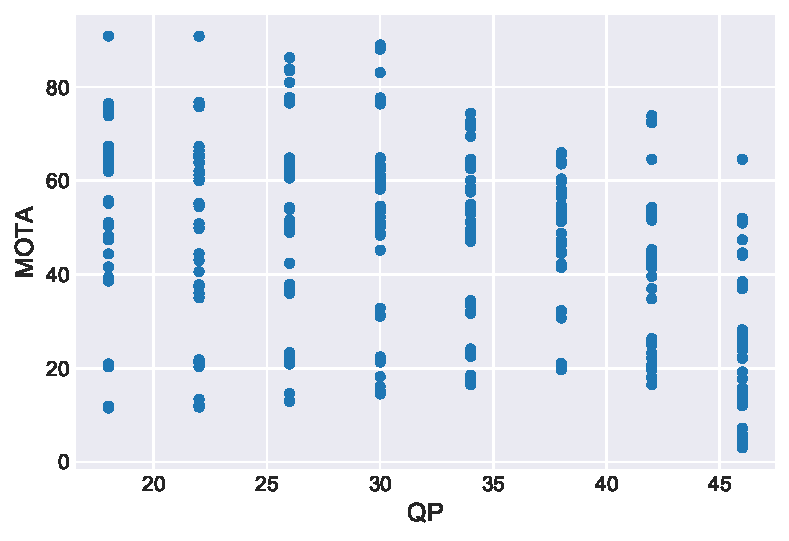
\includegraphics[width=\linewidth]{img/score_transformation_before.pdf}
    \caption{MOTA vs QP scatter plot}
    \label{fig:score_transformation_before}
  \end{subfigure}%
  \begin{subfigure}{.5\linewidth}
    \centering
    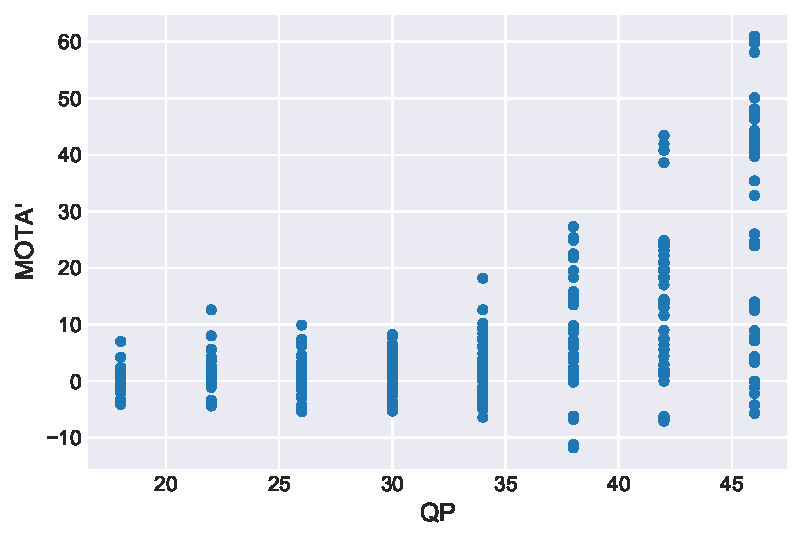
\includegraphics[width=\linewidth]{img/score_transformation_after.pdf}
    \caption{$\text{MOTA}'$ vs QP scatter plot }
    \label{fig:score_transformation_after}
  \end{subfigure}
  \caption[Scatter plots before and after the MOTA transformation for t-test]{%
    Scatter plots before and after the MOTA transformation for t-test.%
  }
  \label{fig:score_transformation}
\end{figure}

To perform t-test, the appropriate hypotheses will be
\begin{equation}
    \begin{aligned}
        H_0 : \mu_{\text{diff}} \leq 0 \\
        H_1 : \mu_{\text{diff}} > 0 \\
    \end{aligned}
\end{equation}
where $\mu_{\text{diff}}$ is the mean of 12 transformed score values $p_{\text{diff}}$. The null hypothesis is the case when the mean $\mu_{\text{diff}}$ is less than or equal to the population mean of 0. The alternative hypothesis is the case when the mean $\mu_{\text{diff}}$ is greater than the population mean of 0. Applying an one-sided t-test for "all" object classes across all the video sequences at a confidence level of 0.05, we obtain the results in Table \ref{tab:t_test_all} using the Python package \cite{virtanen_scipy_2020}. The value less than the significance level of 0.05 is bolded in the table.
\begin{table}[!tb]
    \centering
    \caption[One-sided t-test for "all" object classes across all the video sequences]
    {One-sided t-test for "all" object classes across all the video sequences.}
    \resizebox{1.0\linewidth}{!}{
    
% \begin{tabular}{lllllllllllllllllllll}
\begin{tabular}{ccccccccccccccccccccc}
\toprule
{} &                 IDTP &                 IDFP &                 IDFN &                 IDF1 &            IDP &                  IDR &                Recall &      Precision &                    F1 &                    MT &    PT &                   ML &                    TP &                   FP &                    FN &                  IDs &                   FM &               mAP-50 &                  MOTA &                 MOTP \\
\midrule
p-value(QP=18) &                 0.44 &                 0.90 &                 0.44 &                 0.87 &           0.70 &                 0.90 &                  0.31 &  \textbf{0.02} &                  0.06 &         \textbf{0.05} &  0.79 &        \textbf{0.02} &                  0.29 &                 0.99 &                  0.29 &                 0.98 &                 0.94 &                 0.68 &         \textbf{0.03} &                 0.97 \\
p-value(QP=22) &                 0.91 &                 0.49 &                 0.91 &                 0.79 &           0.71 &                 0.79 &   $\pmb{< |10^{-3}|}$ &  \textbf{0.03} &   $\pmb{< |10^{-2}|}$ &         \textbf{0.02} &  0.63 &        \textbf{0.03} &                  0.39 &                 0.99 &                  0.39 &                 0.92 &                 0.93 &                 0.38 &   $\pmb{< |10^{-2}|}$ &                 0.97 \\
p-value(QP=26) &                 0.16 &                 0.07 &                 0.16 &                 0.58 &           0.91 &                 0.20 &   $\pmb{< |10^{-5}|}$ &           0.89 &   $\pmb{< |10^{-3}|}$ &   $\pmb{< |10^{-3}|}$ &  0.59 &  $\pmb{< |10^{-3}|}$ &   $\pmb{< |10^{-2}|}$ &                 0.27 &   $\pmb{< |10^{-2}|}$ &                 0.53 &                 0.41 &        \textbf{0.02} &   $\pmb{< |10^{-3}|}$ &                 1.00 \\
p-value(QP=30) &                 0.08 &                 0.76 &                 0.08 &                 0.24 &           0.65 &        \textbf{0.03} &   $\pmb{< |10^{-5}|}$ &           0.83 &   $\pmb{< |10^{-2}|}$ &   $\pmb{< |10^{-3}|}$ &  0.50 &  $\pmb{< |10^{-2}|}$ &                  0.10 &                 0.84 &                  0.10 &                 0.29 &                 0.47 &                 0.08 &   $\pmb{< |10^{-3}|}$ &                 0.99 \\
p-value(QP=34) &  $\pmb{< |10^{-2}|}$ &  $\pmb{< |10^{-2}|}$ &  $\pmb{< |10^{-2}|}$ &  $\pmb{< |10^{-2}|}$ &           0.60 &  $\pmb{< |10^{-4}|}$ &   $\pmb{< |10^{-6}|}$ &           1.00 &   $\pmb{< |10^{-4}|}$ &   $\pmb{< |10^{-5}|}$ &  0.95 &  $\pmb{< |10^{-5}|}$ &   $\pmb{< |10^{-3}|}$ &        \textbf{0.01} &   $\pmb{< |10^{-3}|}$ &  $\pmb{< |10^{-3}|}$ &  $\pmb{< |10^{-2}|}$ &        \textbf{0.01} &   $\pmb{< |10^{-4}|}$ &                 0.99 \\
p-value(QP=38) &  $\pmb{< |10^{-3}|}$ &  $\pmb{< |10^{-6}|}$ &  $\pmb{< |10^{-3}|}$ &  $\pmb{< |10^{-4}|}$ &           0.88 &  $\pmb{< |10^{-6}|}$ &   $\pmb{< |10^{-7}|}$ &           1.00 &   $\pmb{< |10^{-6}|}$ &   $\pmb{< |10^{-7}|}$ &  0.92 &  $\pmb{< |10^{-7}|}$ &   $\pmb{< |10^{-4}|}$ &  $\pmb{< |10^{-4}|}$ &   $\pmb{< |10^{-4}|}$ &  $\pmb{< |10^{-2}|}$ &  $\pmb{< |10^{-2}|}$ &  $\pmb{< |10^{-3}|}$ &   $\pmb{< |10^{-5}|}$ &                 0.57 \\
p-value(QP=42) &  $\pmb{< |10^{-5}|}$ &  $\pmb{< |10^{-4}|}$ &  $\pmb{< |10^{-5}|}$ &  $\pmb{< |10^{-6}|}$ &           0.17 &  $\pmb{< |10^{-7}|}$ &  $\pmb{< |10^{-10}|}$ &           1.00 &   $\pmb{< |10^{-8}|}$ &   $\pmb{< |10^{-9}|}$ &  0.40 &  $\pmb{< |10^{-6}|}$ &   $\pmb{< |10^{-8}|}$ &  $\pmb{< |10^{-5}|}$ &   $\pmb{< |10^{-8}|}$ &  $\pmb{< |10^{-3}|}$ &                 0.12 &  $\pmb{< |10^{-5}|}$ &   $\pmb{< |10^{-8}|}$ &        \textbf{0.01} \\
p-value(QP=46) &  $\pmb{< |10^{-8}|}$ &  $\pmb{< |10^{-4}|}$ &  $\pmb{< |10^{-8}|}$ &  $\pmb{< |10^{-9}|}$ &  \textbf{0.04} &  $\pmb{< |10^{-9}|}$ &  $\pmb{< |10^{-13}|}$ &           0.23 &  $\pmb{< |10^{-12}|}$ &  $\pmb{< |10^{-13}|}$ &  0.69 &  $\pmb{< |10^{-8}|}$ &  $\pmb{< |10^{-11}|}$ &        \textbf{0.02} &  $\pmb{< |10^{-11}|}$ &  $\pmb{< |10^{-2}|}$ &        \textbf{0.01} &  $\pmb{< |10^{-9}|}$ &  $\pmb{< |10^{-11}|}$ &  $\pmb{< |10^{-3}|}$ \\
\bottomrule
\end{tabular}

    }
\label{tab:t_test_all}
\end{table}
From this result, for example, the MOTA score at QP = 18 is significantly lower than the score at the uncompressed sequence with 95\% confidence as we reject the null hypothesis. In fact, we can conclude for most of the metrics except Precision and PT that the performance score is either greater or less than the score at the uncompressed case with 95\% confidence. From Figure \ref{fig:averaged_result_all_multiplots_qp}, the Precision score increases first and then decrease as QP increases. Therefore, the result from the t-test is consistent with the the visualization. According to Equation \ref{eqn:Precision}, Precision depends on TP and FP, and increase of p-value can be confirmed at QP = 30. The detailed reasoning for this outcome is explained in the following section \ref{sec:results/section_b}. A slight increase of MOTP can also be confirmed from QP = 26. We also applied an one-sided t-test to the "person" object class and the similar conclusions can be made. See Appendix \ref{sec:appendix/section_t_test_0} for the "person" object case.

As we just showed the results from the visualization and the statistical analysis for the multiple video sequences, most metrics results in a way as expected but the outcomes of Precision and MOTP were not entirely expected. We will further analyze individual sequences in the next section.


% As \cite{sharrab_modeling_2017} shows that bitrate is inversely proportional to QP and HEVC range from 0 to 51 \cite{sullivan_overview_2012}, our proposed formula 